\section{はじめに}

\begin{figure}[!b]
\centering
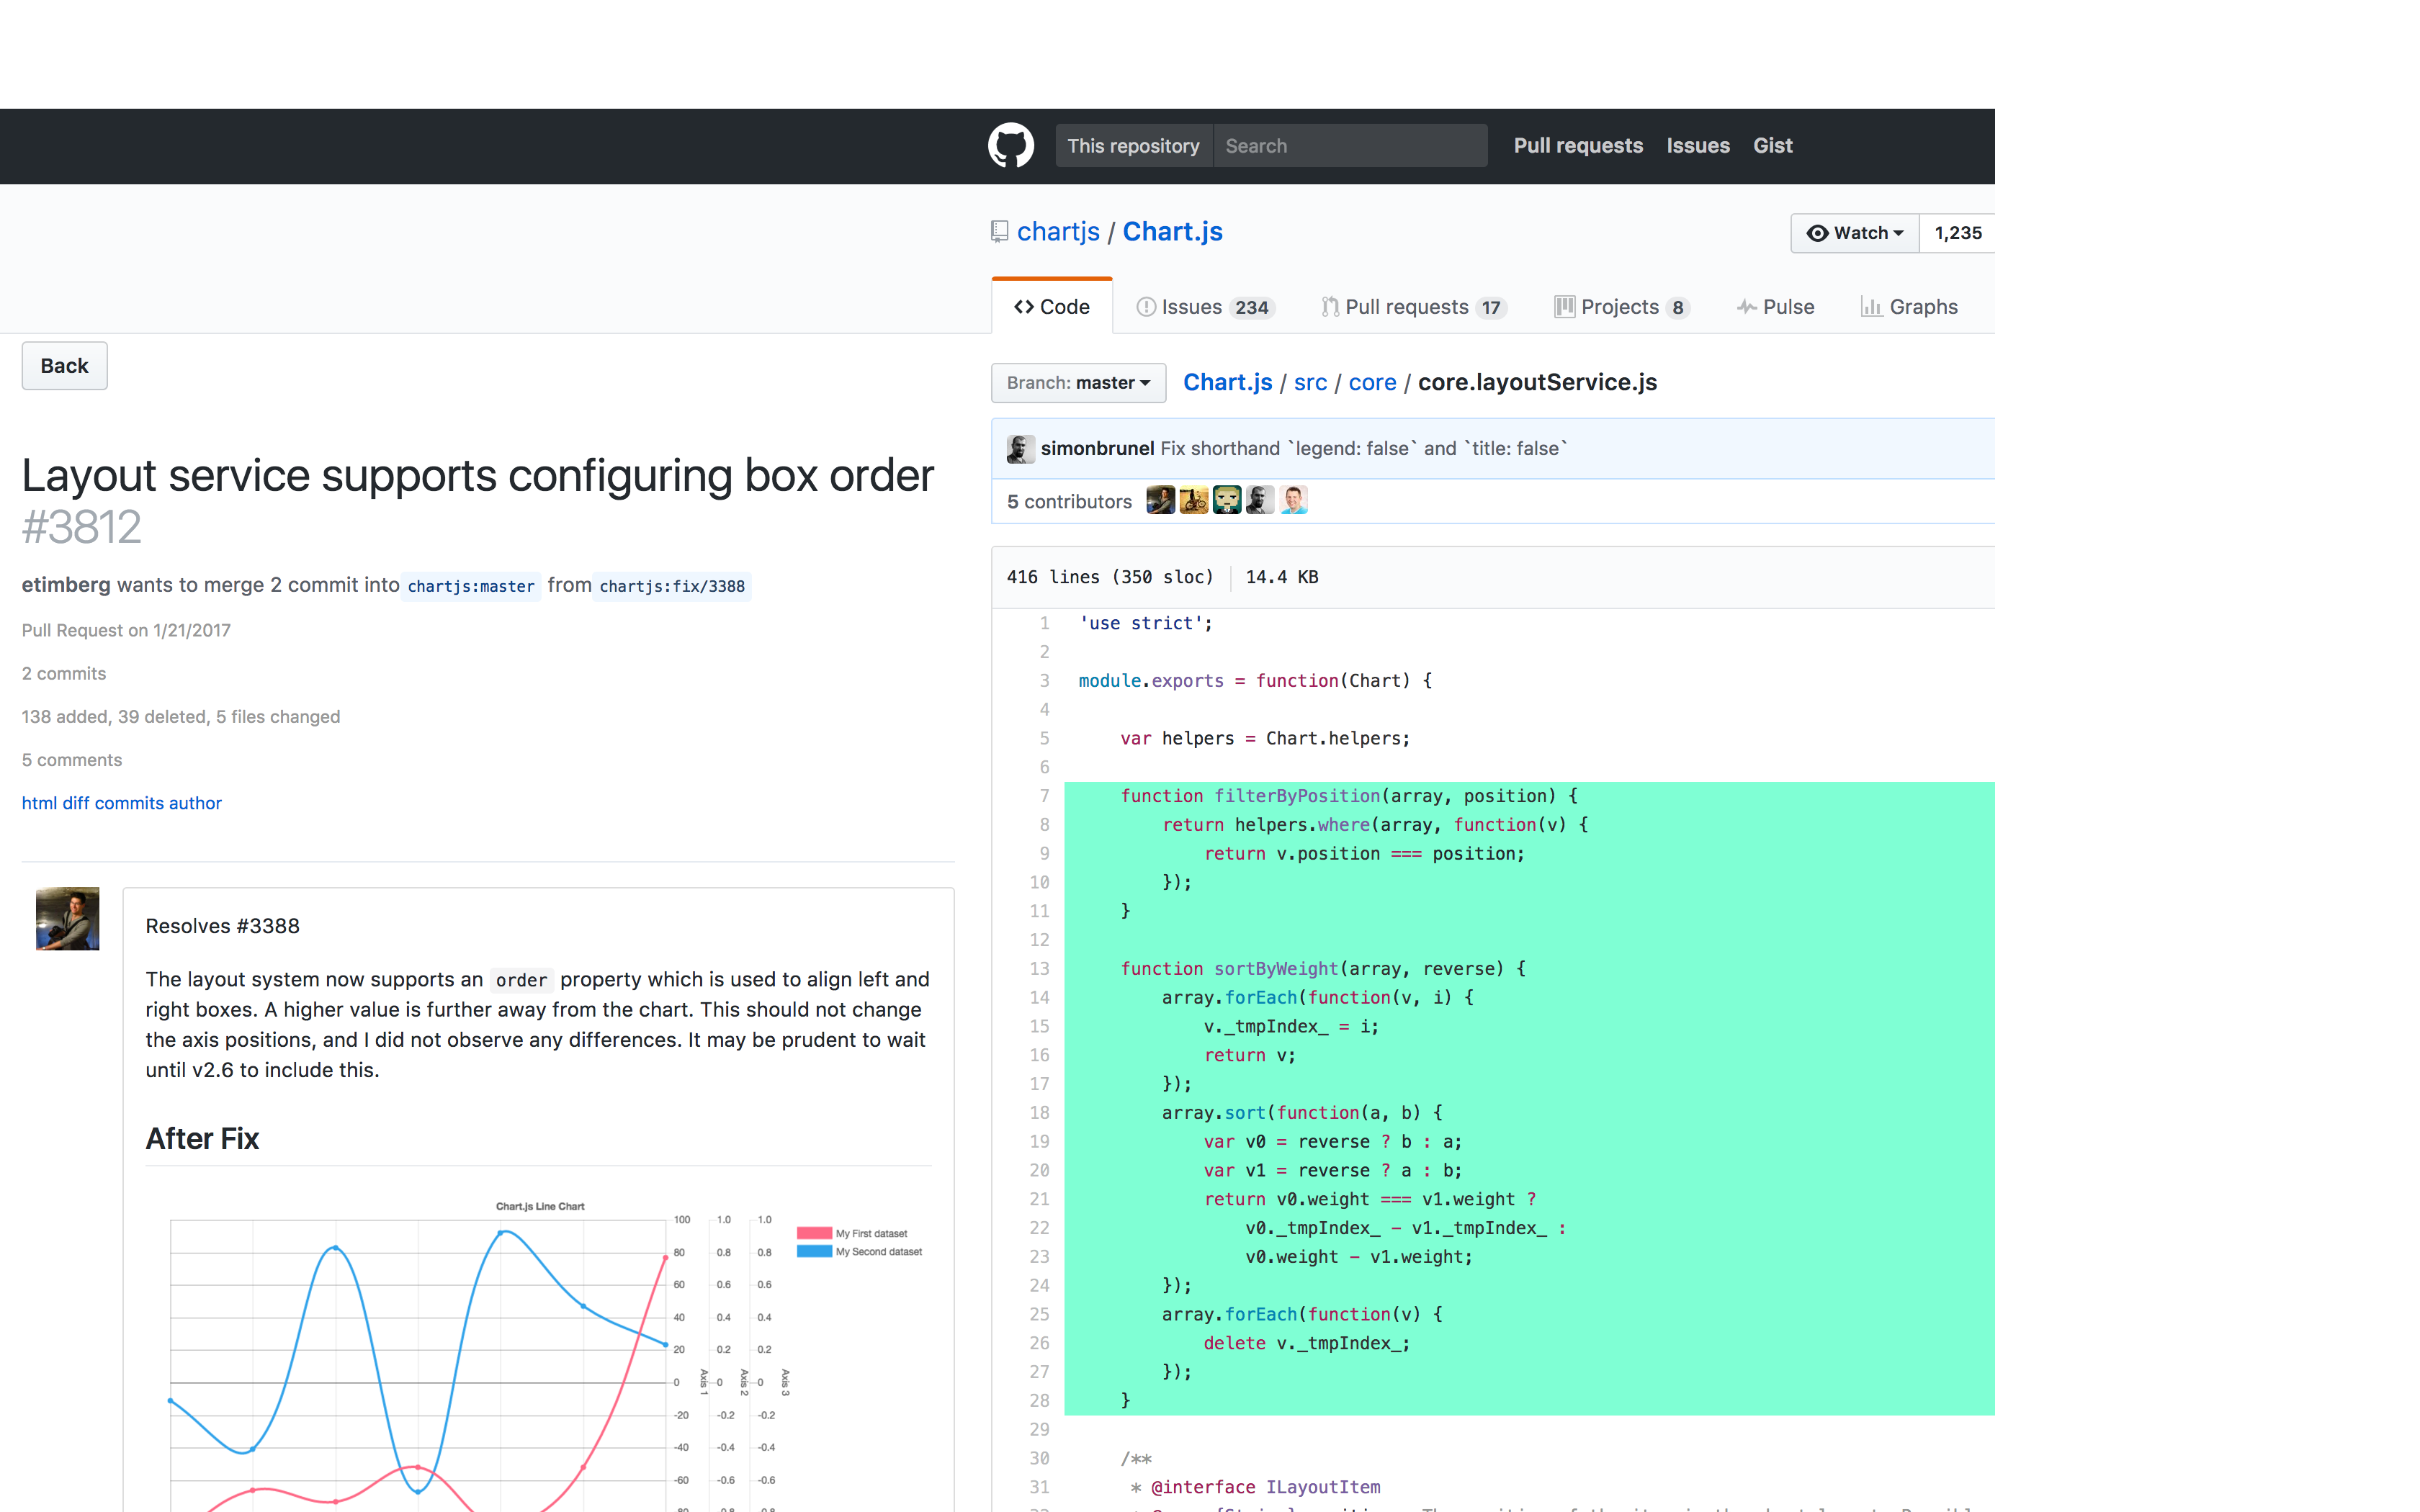
\includegraphics[width=1.2\columnwidth]{interface/top_image.png}
\caption{CodeGlass上でユーザは選択したコード断片に関連する過去のプルリクエストを参照することができる.プルリクエストの説明文に含まれる実装内容や開発背景といった情報は,ユーザのコード理解を支援することができる.}
~\label{fig:top}
\end{figure}

ソフトウェア開発においてソースコードの理解は必要不可欠である.
ソフトウェア開発者はコードを書くだけでなく,同じチームの他の開発者によるコード変更をレビューしたり,開発プロジェクトのスケジュールや進捗を管理したりする必要がある.
その全てのタスクにおいて,正確なコード理解が常に必要となる.
このため,ソフトウェア開発におけるコード理解の重要性は広く認知されている.

% Code comprehension is critical in software development.
% Developers' work includes not only writing code, but also reviewing bug fixes by other team members, managing projects, and examining potentially useful libraries.
% Correct code understanding is necessary to successfully complete these tasks.
% Code comprehension support, thus is, of great interest to programmers and project managers.




実際のソフトウェア開発では,ソースコード全体ではなく,コードの一部分(コード断片)の理解が必要となることが多い.
例えば,開発者はバグを修正するために,関連するコード断片(関数やクラスなど)の現状を把握してからコードの修正を行う.
コードレビューにおいても同様に,主に変更のあったコード断片に対して問題がないことを確認する.
このようにコード断片の理解はソフトウェア開発において重要であり,コード断片の実装内容や開発背景といった情報をユーザに提供することができれば,ソフトウェア開発を支援できると考えられる.
%しかし,既存のシステムではコード断片に関連する有用な情報をユーザに提供できていない.


% In practice, developers frequently need to understand a portion of code, or \textit{a code piece}, rather than the entire project.
% For instance, they are asked to fix a bug for part of code (e.g., a function or class).
% Code review is another activity that requires an understanding of code pieces.
% Information relevant to the given code piece (e.g., logs of revisions and reviews) can facilitate code comprehension by providing its development background.
% Despite these apparent needs, existing systems and tools do not assist developers to acquire such information for code pieces well.

近年のソフトウェア開発では,GitHub\footnote{\url{https://github.com}}という多人数開発を支援するコードホスティングサービスが広く利用されている.
GitHubでは,コード変更の管理とコードレビューを支援する機能であるプルリクエストを用いたソフトウェア開発が推奨されている.
他の開発者にコード変更の意図や内容を正しく伝えるためには,プルリクエストにコード変更の説明文を記すことが重要とされている.
この説明文には,コード変更の実装内容や開発背景といった,コード変更を理解するための情報を記載することが求められる.
我々が行ったプログラマを対象としたインタビュー調査では,プルリクエストに含まれる情報がコード断片の理解において有用であることが示唆された.
しかし,プルリクエストは主にソフトウェア開発の効率化を目的として利用されており,コード断片の理解を支援するためには十分に活用されていない.

% Recent software projects commonly use GitHub, a web service that supports collaborative and distributed development.
% GitHub encourages software development using pull requests.
% A pull request is a method for submitting code changes with descriptions.
% GitHub also provides features that manage a review process through pull requests.
% Many projects actively use pull requests, and developers include information about code changes in them.
% Our formative study found that pull requests have a potential to serve as a useful information resource to facilitate code understanding.
% However, existing pull request retrieval tools are not necessarily effective for code comprehension purposes.
% This observation motivates us to design an interface to support comprehension of code pieces using relevant pull requests and examine its effect.
%This observation motivates us to design an interface to support comprehension of code pieces by making relevant pull request more accessible to developers and examine its effect.



そこで本研究では,コード断片に関連する情報を提供するCodeGlassというシステムを開発した(図\ref{fig:top}).
CodeGlassはユーザが選択したコード断片に関連する過去のプルリクエストを抽出し,ユーザに提供する.
さらに,プルリクエストの説明文を解析し,実装内容や開発背景に関する文章をインターフェース上で強調して表示することが可能となっている.
LHDiff~\cite{LHDiff}を改良したアルゴリズムにより,選択されたコード断片が過去のバージョンにおいて分裂していた場合にも,CodeGlassは関連する過去のプルリクエストを提供することができる.
学生によるCodeGlassの定量的評価により,コード断片の理解のための情報収集において,CodeGlassが有用であることが分かった.
さらにプログラマを対象とした定性的評価を行った結果,専門的用途におけるCodeGlassの有用性が明らかとなった.
本研究がソフトウェア工学とヒューマン・コンピュータ・インタラクションの分野にもたらす貢献は以下の通りである.

% In this paper, we present an interactive piece-level code examination tool, called CodeGlass.
% The system extracts pull requests and review comments associated with the chosen code piece.
% We employ the LHDiff algorithm~\cite{LHDiff} with modifications to identify past commits and pull requests related to the chosen code piece.
% Our modification allows the algorithm to find code piece changes more accurately even if they are split in the previous commit.
% Our user study revealed that CodeGlass effectively supported participants to acquire information about implementation rationales and development history.


% This work offers the following contributions to the fields of Human-Computer Interaction and software engineering:

\begin{itemize}
% \setlength{\leftskip}{-3mm}
\item ユーザが選択したコード断片に関連する過去のプルリクエストを表示し,実装内容や開発背景に関する文章を強調するCodeGlassインターフェースの構築
\item LHDiff~\cite{LHDiff}の改良による,過去のバージョンにおけるコード断片の追跡精度の向上
\item コード断片の理解におけるCodeGlassの有用性の定量的・定性的評価
\end{itemize}


% \begin{itemize}
% \setlength{\parskip}{1mm}
% \setlength{\itemsep}{0mm}
% \setlength{\leftskip}{-3mm}
% \item \textbf{CodeGlass interface}: It supports piece-level code examination and allows developers to view descriptions and review comments in past pull requests associated with the chosen code piece.
% \item \textbf{LHDiff algorithm modifications}: We modify LHDiff~\cite{LHDiff} with a graceful matching mechanism. Our evaluation revealed that our algorithm can backtrack changes on a code piece at high precision and recall.
% \item \textbf{CodeGlass user evaluations}: Our lab study uncovers improved performance on acquiring implementation rationales and development history. Our informal expert review confirmed various potential use scenarios of CodeGlass in professional development environments.
% \end{itemize}





